% AEJ-Article.tex for AEA last revised 22 June 2011
\documentclass[PP]{AEA}

%%%%%% NOTE FROM OVERLEAF: The mathtime package is no longer publicly available nor distributed. We recommend using a different font package e.g. mathptmx if you'd like to use a Times font.
\usepackage{mathptmx}

% The mathtime package uses a Times font instead of Computer Modern.
% Uncomment the line below if you wish to use the mathtime package:
%\usepackage[cmbold]{mathtime}https://www.overleaf.com/project/5de54d6638f785000167866a
% Note that miktex, by default, configures the mathtime package to use commercial fonts
% which you may not have. If you would like to use mathtime but you are seeing error
% messages about missing fonts (mtex.pfb, mtsy.pfb, or rmtmi.pfb) then please see
% the technical support document at http://www.aeaweb.org/templates/technical_support.pdf
% for instructions on fixing this problem.

% Note: you may use either harvard or natbib (but not both) to provide a wider
% variety of citation commands than latex supports natively. See below.

% Uncomment the next line to use the natbib package with bibtex 
\usepackage{url}
\urlstyle{same} % makes the font the same
\usepackage{natbib}
\usepackage{hyperref}
\usepackage{acronym}
\usepackage[names]{xcolor}
\usepackage{graphicx}
\usepackage{csvsimple}
% Uncomment the next line to use the harvard package with bibtex
%\usepackage[abbr]{harvard}
\usepackage{etoolbox}
\usepackage{geometry}
\usepackage{caption} % to re-use counters
\usepackage{threeparttable}

\newtoggle{fancy}
\togglefalse{fancy}

\newtoggle{draft}
\toggletrue{draft}
%\togglefalse{draft}

\newtoggle{final}
%\togglefalse{final}
\toggletrue{final}
%\iftoggle{final}{\togglefalse{draft}}{}


\iftoggle{draft}{
\usepackage{draftwatermark}
\SetWatermarkText{DRAFT}
\SetWatermarkScale{0.5}
\SetWatermarkLightness{0.85}%
}{\usepackage[final]{draftwatermark}}

\usepackage{xspace}
% to adjust floats
\usepackage{placeins}
% to read the table
\usepackage{booktabs}
\usepackage{ifthen}
\usepackage{csvsimple}
\usepackage{longtable}

\usepackage{textcomp}

\iftoggle{fancy}{
\input{fancy-config.tex}
}{}

\iftoggle{final}{
\usepackage[disable]{todonotes}
\newcommand{\misscitep}[2]{\citep{#2}}
\newcommand{\misscitet}[2]{\citet{#2}}
}{
\usepackage{todonotes}
\geometry{verbose,letterpaper,
	tmargin=1in,bmargin=1in,lmargin=1in,rmargin=2in}
\setlength{\marginparwidth}{1.9in}
\newcommand{\misscitep}[2]{\todo[color=green]{Missing citation: #1}{(\textcolor{red}{#2})}}
\newcommand{\misscitet}[2]{\todo[color=green]{Missing citation: #1}{\textcolor{red}{#2}}}
}



% This command determines the leading (vertical space between lines) in draft mode
% with 1.5 corresponding to "double" spacing.
\draftSpacing{1.5}

%% make somewhat tigher enumeration environments
\usepackage{enumitem}
\setlist[enumerate]{itemsep=0pt,parsep=0pt,topsep=1pt}
\setlist[itemize]{itemsep=0pt,parsep=0pt}

%% Acronyms
\acrodef{AEA}{American Economic Association}
\acrodef{DOI}{Digital Object Identifier}
\acrodef{FAIR}{Findable, Accessible, Interoperable, Re-usable}
\acrodef{PSID}{Panel Study of Income Dynamics}
\acrodef{HRS}{Health and Retirement Study}
\acrodef{RCT}{randomized control trial}
\acrodef{ICPSR}{Inter-university Consortium for Political and Social Research}
\acrodef{DCAP}{data and code availability policy}
\acrodef{PAP}{pre-analysis plans}
\acrodef{NACJD}{National Archive of Criminal Justice Data}
\acrodef{IAB}{Research Data Center (FDZ) at the Institute for Employment Research}
\acrodef{FSRDC}{Federal Statistical Research Data Centers}
\acrodef{FAQ}{frequently asked questions}
\acrodef{ReStud}{Review of Economic Studies}
\acrodef{EJ}{Economic Journal}
\acrodef{JASA}{Journal of the American Statistical Association}
\acrodef{CJE}{Canadian Journal of Economics}
\acrodef{AJPS}{American Journal of Political Science}
\acrodef{PII}{personally identifiable information}
\newcommand{\aeadcr}{AEA Data and Code Repository}

% reset colors
\definecolor{darkblue}{rgb}{0 0 255}
\hypersetup{colorlinks,breaklinks,citecolor=darkblue,linkcolor=darkblue,urlcolor=darkblue}

% Different ways to cite URLS
%\newcommand{\urlcite}[2]{\href{#1}{#2}
\newcommand{\urlcite}[2]{#2\footnote{\url{#1}}}
\newcommand{\purlcite}[2]{#2.\footnote{\url{#1}}}
\newcommand{\furlcite}[2]{#2 (\url{#1})}

%
% Periods covered by the report 
% Should be read in from R
\newcommand{\version}{Sun Dec 13 21:14:12 2020}
\newcommand{\firstday}{2019-12-01}
\newcommand{\lastday}{2020-11-30}
\newcommand{\jiraissues}{832}
\newcommand{\jiramcs}{509}
\newcommand{\jiraissuescplt}{715}
\newcommand{\jiramcscplt}{402}
\newcommand{\jiraexternal}{36}
\newcommand{\jiramcsexternal}{27}
\newcommand{\jiramcspending}{307}
\newcommand{\pkgsizemean}{1.72}
\newcommand{\mcpubtotal}{345}
\newcommand{\mcpubincmplt}{5}
\newcommand{\pppubnoncompl}{1}
\newcommand{\mcpubnoncompl}{1}
\newcommand{\pkgsizeq50x}{0.02}
\newcommand{\pkgsizeq90x}{6.47}


%\renewcommand{\firstday}{Dec 1, 2019}
%\renewcommand{\lastday}{Nov 30, 2020}

\begin{document}

\title{Report for 2020 by the AEA Data Editor }
\shortTitle{Report by Data Editor}
\author{Lars Vilhuber\thanks{%
Cornell University, lars.vilhuber@cornell.edu. }
}
\date{\today}
\pubMonth{May}
\pubYear{2020}
\pubVolume{--}
\pubIssue{--}
\JEL{}
\Keywords{reproducibility; replicability; science of science}




\maketitle

The \ac{AEA} Data Editor's  mission is to ``design  and  oversee  the  AEA  journals’  strategy for archiving and curating research data and promoting  reproducible  research'' \citep{10.1257/pandp.108.745}. The 2018 Report by the Data Editor \citep{10.1257/pandp.109.718} articulates how to implement that mission. Since July 2019, we have conducted comprehensive pre-publication reproducibility checks for all regular AEA journals, developed guidance for authors, and worked with peers at societies and groups in economics and elsewhere. 

Based on the experience from the first full year of reproducibility verification, we implemented several improvements in mid-2020. We provided improved guidance to authors depositing materials, clarified the \ac{DCAP}, expanded and clarified additional policies on third-party reproducibility checks, on post-publication updates to replication packages, and on required replication materials for field and lab experiments  (Section~\ref{sec:dcap}). We have reached out to numerous data creators and providers --- both authors who have created unique data resources, and commercial data providers that often provide the data for economic research --- and have discussed with these data providers access to data for reproducibility checks, mechanisms to request publication approval, and generally informed them of the need for reproducibility, provenance tracing, and transparency in economic research (Section~\ref{sec:producers}). 
We continue to coordinate with other journals, societies, and registries on these topics (Section~\ref{sec:coordination}).


\section{Updating the AEA Data and Code Availability Policy}
\label{sec:dcap}

After having introduced stronger principles of provenance and transparency into the  \ac{AEA}'s data and code availability policy in 2019 \citep{10.1257/pandp.110.dcap}, we monitored compliance and understanding as evidenced by the replication package submissions we received. It became quickly clear that stronger guidance, and greater clarity were needed to assist authors in complying with the \ac{DCAP}. Authors struggled with how best to document their code and data,  with the process of deposing data and code, and the ability to provide clear data provenance, including  data citations. We clarified the policy, and released the revised version in September 2020. The main content remains unchanged, but we simplified the main policy,  separated out the policy as applied to papers conducting (field and lab) experiments, and expanded the policy to encompass more clearly any primary data collection. We also introduced  supplementary policies that lay out how and when we expect reproducibility checks by third-parties to be conducted (also see \hyperref[sec:3rdparty]{our interactions with third-party verifiers}, and, as a logical consequence of more transparent data and code deposits, how to revise data and code deposits when post-publication changes become necessary. These policies are reprinted in \citet{10.1257/pandp.111.dcap} and accessible online at \url{https://www.aeaweb.org/journals/data}.

We also clarified the data and code availability policy as it applies to papers submitted to these Proceedings. All empirical and computational articles in the proceedings need to make code and data available in the same AEA Data and Code Repository as articles in the journals. However, other than verifying compliance with the policy (materials were deposited) and conducting basic checks (material can be read, metadata is in order), we do not conduct the same pre-publication reproducibility checks as we do for regular articles (see Section \ref{sec:compliance} for statistics on compliance).

But policies only outline what should occur, not how authors can achieve compliance. In order to assist authors in complying with the policy, thus improving turnaround times, we developed more detailed step-by-step guidance at \href{https://aeadataeditor.github.io/aea-de-guidance/step-by-step.html}{aeadataeditor.github.io/aea-de-guidance/step-by-step.html}. We also revised the information that authors need to provide when their manuscript is conditionally accepted (or, in some cases, during the review process). We have eliminated the duplicative requirement to provide  README files during the manuscript submission process --- they remain a required element in the data and code deposit process --- replacing it with a simpler form that requires authors to attest to compliance of their manuscript with the data citation requirement, provide details on where the data and code were deposited, and has them alert the Data Editor to any constraints on data access\footnote{The form is available at \href{https://www.aeaweb.org/journals/forms/data-code-availability}{aeaweb.org/journals/forms/data-code-availability}.} At the same time, the form provides hyperlinks to the guidance mentioned above. A simplified version of the form (reduced to a few checkboxes) is incorporated into the initial manuscript submission workflow. The primary goal of these forms and checkboxes is to alert authors to the need to comply with the policy early on, and hopefully leading to better compliance by the time that manuscripts are conditionally accepted. 

Furthermore, in collaboration with data editors at other journals in economics, management, and statistics, we have released a template README \citep{READMEv1.0.0} which helps authors compile all the information required for complete documentation of their data and code deposit.\footnote{The README is available at \href{https://social-science-data-editors.github.io/template_README/}{social-science-data-editors.github.io/template\_README/}.} With the publication of this report in the Proceedings, we will start verifying that authors use the README to document their replication package.


\subsection{Improving Findability of Replication Materials at the AEA}
\label{sec:findability}

Since the AEA began using a data and code repository hosted by \ac{ICPSR}, all deposits have JEL codes, and authors can add funder information and key metadata describing the data that is available within the deposit. Many authors avail themselves of this option. These attributes aid in making each deposit  findable through scholarly search engines such as \urlcite{https://clarivate.com/webofsciencegroup/solutions/web-of-science/}{Web of Science} and \urlcite{https://scholar.google.com/}{Google Scholar}. 

Deposits made prior to July 2019 and since migrated to the AEA Data and Code Repository do not have the rich metadata, since it must be entered interactively by authors. To improve the metadata of older deposits, we ran a campaign in summer and fall of 2020, thanks to the support provided by a research team at the University of Michigan and ICPSR. This campaign targeted several hundred papers, providing authors with a tool to augment the metadata associated with their deposits. A report on the success of the campaign is forthcoming, and the metadata provided by the authors is being incorporated as this report was being compiled. A second campaign will complete the work in Spring or Summer of 2021. 

Deposits receive their own \ac{DOI}, and can be cited in line with the Data Citation Principles \citep{Altman2013-fl,jddcp}. Authors are required to explicitly cite their data supplement if it contains original data; an entry in the references is automatically added in all cases. Conversely, the article that a supplement is associated with is clearly identified on the supplement's landing page. Future enhancements to the platform will be able to display other articles that also cite a supplement. 

We continue to verify that authors cite the datasets they have used and accessed, as required by the \ac{DCAP}, the AEA's citation requirements, and in line with the Data Citation Principles.  Data citations increase findability of data, allow data providers to receive proper credit, and align the Association with broader principles in the academic publishing world. The AEA's  \urlcite{https://www.aeaweb.org/journals/policies/sample-references}{Sample References} provide a style reference, and additional guidance for non-standard data sources, such as confidential or proprietary data, has been developed in collaboration with other journals and guidance by librarians.\footnote{\url{social-science-data-editors.github.io/guidance/addtl-data-citation-guidance.html}}.


\subsection{Third-party repositories}

The \ac{DCAP} allows for code and data deposit to be deposited at other trusted repositories, as long as all other elements of the \ac{DCAP} are complied with. In fact, authors are discouraged from duplicating deposits they have made elsewhere in the \aeadcr{}. This is intended to allow others to create replication packages prior to submitting at the AEA's journals, as a component of a reproducible workflow and possibly in compliance with funder data management policies. We have not observed many authors availing themselves of this possibility, with probably less than 10 deposits made in such a way. Authors wishing to deposit replication packages early in the research lifecycle are encouraged to consult the Social Science Data Editors website, where links to trusted repositories are provided.
	
\subsection{Post-publication modifications}

At the time of publication, the article is linked with one (or more) archived supplements, constituting the version of record. What happens when, despite pre-publication scrutiny, an error in the code emerges? The \ac{DCAP} provides for a clear policy on which modifications constitute a minor edit to the version of record, and which modifications lead to a higher version number, without modification of the existing version of record. In particular, any change that potentially changes a computational result will lead to a new version of the deposit being created, without changing or removing the version of record, even if the modifications fixes an error. However, the presence of replication packages that are newer than the version of record is signalled to readers via a banner, and is recorded in the metadata.

\subsection{Intellectual Property and Licenses} 
\label{sec:ip}

For new deposits at the \aeadcr{}, authors retain  copyright. The default license for all repositories based at openICPSR is the  Creative Commons Attribution (CC-BY) \citep{CreativeCommons2017}, but authors can choose their own license,  though such licenses will be vetted by the Data Editor for compliance with the \ac{DCAP}. We see few authors deviate from the standard license. When deviating, authors tend to choose a different, open source license \citep{OpenSourceInitiative2018} for software and code. In a very small number of cases, we have worked with authors to publish data under more restrictive licenses, due mostly to ethical concerns, while ensuring that replication remains possible.

% Dwayne Benjamin, Toronto/P&P
% AER/FL Police officers

\subsection{Compliance}
\label{sec:compliance}

\begin{table}[t]
    \centering
    \caption{Compliance}
    \label{tab:compliance}
    \begin{threeparttable}
    \begin{tabular}{lccc}
    \toprule
         & Compliant & Incomplete & Non-compliant \\
    \midrule
    Papers and Proceedings &  87    &  4 & 1\\
    AER and journals       & xx    &  1  & 0\\
    \bottomrule
    \end{tabular}
    \begin{tablenotes}
    \footnotesize
    \item[] \textit{Note}: Unit of observation are manuscripts assessed between \firstday{} and \lastday{}. ``Incomplete" means the data deposit has not been completed, though the article has been published. ``Non-compliant" means that code or other required materials have not been provided.
    \end{tablenotes}
    \end{threeparttable}
\end{table}


Authors have been very compliant with the policy (Table~\ref{tab:compliance}). We note that authors can be compliant with the policy without providing a copy of the data, as long as the reason for the inability to provide the data is acceptable, correct, and documented as part of the replication materials. In some cases, we have requested data that was not initially provided, when such data could be legally and ethically provided; by the second round of assessments, compliance was generally achieved (see also our discussion of outreach to data providers). In a very small number of cases, authors having conducted research in restricted-access data environments did not provide code. In several cases, relying on personal experience or by reaching out to the managers of the restricted-access environment, we were able to inform the authors of their ability to provide code, in compliance with any security requirements of the restricted-access data environment. In several cases, authors were unable to access the restricted-access environment due to COVID-19 lockdowns, which we accommodated in various ways; however, in all cases, code was ultimately provided. For a very small number of articles, compliance was achieved after the manuscript had been published. We are aware of only one case where the authors were unable to provide code because their employer asserted copyright and did not give permission to post code. One case in which the manuscript has been published is currently pending corrections by the authors, and has not been published as of \today, one month after publication of the article.

\begin{center}
    No changes beyond here
\end{center}

\section{Infrastructure for Reproducibility}
\label{sec:infrastructure}

The Data Editor manages the infrastructure needed to access data and code, conduct reproducibility checks, and archive and preserve replication packages. The first two points are provided by the replication team at Cornell University, the latter primarily by the  \aeadcr{} provided by openICPSR at the University of Michigan, with additional support from the AEA's in-house IT staff. 


\subsection{Pre-publication verification of computational reproducibility}
\label{sec:verification}


\begin{quote}
Report on articles (manuscript ID), reports (unique issues = tasks) and published repositories (only when tied to an article, requires transforming manuscript ID into DOI and querying crossref). Redo analysis from 2019.

\end{quote}

\paragraph{The process}

Pre-publicaton verification is conducted by the Data Editor's team at Cornell University. 
Requests for assessment of reproducibility are received, assigned to a team member, who then assesses data availability and compliance with requirements. When some data is available, a full or limited reproducibility check is conducted. If we cannot obtain access to the data or computational resources in a timely fashion, we may reach out to third-parties who can, and request a reproducibility check from them. Once all computations have been completed, a process that can take anywhere from a few minutes to several weeks, a report is compiled, reviewed and approved by the Data Editor, and submitted back to journal editors, who handle most communications with the authors. The report will have  one of four possible recommendations (see Table). A ``conditional acceptance'' implies that a revision will need to be resubmitted to the Data Editor to address any identified shortcomings. An ``acceptance'' means that no further changes are necessary, and both the manuscript (after copy-editing) and the replication package can be scheduled for publications.\footnote{Manuscript and replication package are generally published at the same time, though at the request of either editors or authors, the replication package can be published at any time after acceptance.} However, to streamline processing, we may also recommend an ``acceptance with modifications requested.'' In such a case, the remaining modifications are minor, and can be handled during copy-editing (for instance, a small number of tables need minimal changes) and prior to publication of the replication package (for instance, a fixable error in a program, or a clarification in the README, not affecting any important tables or figures). We have increasingly made use of this feature. While we monitor that authors comply with the request for modifications, no further computational assessment is made. Finally, we may recommend a ``revise and resubmit'' when serious issues have been identified that materially affect the conclusions of the manuscript. In the past year, two manuscripts required conversations with the editors and the authors, and both were resolved to the satisfaction of all involved.

\begin{table}[t]
    \caption{Response options for recommendations}
    \label{tab:responses}
    \centering
    \begin{tabular}{lr}
    \toprule
               & Frequency \\
               \midrule
        Accept &  \\
        Accept with changes &\\
        Conditional accept &\\
        Revise-and-resubmit & \\
        \bottomrule
    \end{tabular}
\end{table}

\paragraph{Metrics}

Between \firstday{}, and \lastday{}, the AEA Data Editor team  handled
\jiraissues{} requests,  for \jiramcs{} manuscripts. Requests typically are channeled to the team by the AEA's journal submission and review system, but others were initiated by authors or editors directly, often while preparing the replication materials. Of these,  responses \jiraissuescplt{} (\jiramcscplt{} manuscripts) were submitted back to editors, and \jiramcspending{} were completed up to the point of publication of the data deposit, including any post-acceptance modifications. A total of \jiraexternal{} issues were sent to external parties with requests for verification (this includes revisions), for \jiramcsexternal{} manuscripts. Table~\ref{tab:jirastats} breaks these numbers down by journal.
%

\begin{table}[]
    \caption{Stats}
    \label{tab:jirastats}
    \begin{threeparttable}
    \centering
    
% Table created by stargazer v.5.2 by Marek Hlavac, Harvard University. E-mail: hlavac at fas.harvard.edu
% Date and time: Sun, Dec 13, 2020 - 10:08:29 PM
\begin{tabular}{@{\extracolsep{5pt}} ccccccccc} 
\toprule 
 & Journal & Issues (rcvd) & Manuscripts (rcvd) & Issues (cplt) & Manuscripts (cplt) & Manuscripts (ext.) & Issues (external) & Manuscripts (pend.) \\ 
\midrule 1 & AEA P&P & 91 & 91 & NA & NA & NA & NA & 86 \\ 
2 & AEJ:Applied Economics & 125 & 63 & 106 & 60 & 2 & 2 & 41 \\ 
3 & AEJ:Economic Policy & 139 & 74 & 113 & 64 & 8 & 13 & 52 \\ 
4 & AEJ:Macro & 150 & 68 & 125 & 64 & 2 & 3 & 44 \\ 
5 & AEJ:Micro & 92 & 45 & 77 & 44 & 3 & 4 & 33 \\ 
6 & AER & 205 & 110 & 171 & 101 & 10 & 12 & 78 \\ 
7 & AER:Insights & 56 & 31 & 52 & 30 & NA & NA & 25 \\ 
8 & JEL & 35 & 20 & 31 & 17 & 1 & 1 & 16 \\ 
9 & JEP & 30 & 20 & 27 & 18 & NA & NA & 13 \\ 
\bottomrule 
\end{tabular} 

    \end{threeparttable}
\end{table}

\begin{comment}
We collected metrics from the online system.%
\footnote{Data  can be found at \citet{E117876V1}.}
Figure~\ref{fig:pre:assessments_journal} shows the distribution of  assessments across journals. Figure~\ref{fig:pre:rounds} shows the number of rounds that the \jiramcs{} completed manuscripts have gone through. Assessment take varying amounts of time, depending on the complexity of the paper and the code. Figure~\ref{fig:pre:round_length} shows the distribution of the time it takes to complete each round of assessment. The distribution of the total length of all revision rounds, from the first submission (to the Data Editor) to final acceptance, is shown in Figure~\ref{fig:pre:revision_length}. Figure~\ref{fig:pre:author_response_time} shows the component of the total length that is due to author response time, i.e., the time between the filing of a report by the AEA Data Editor requesting changes, and the time the manuscript is re-assigned to the AEA Data Editor. 

\begin{figure}
    \centering
%    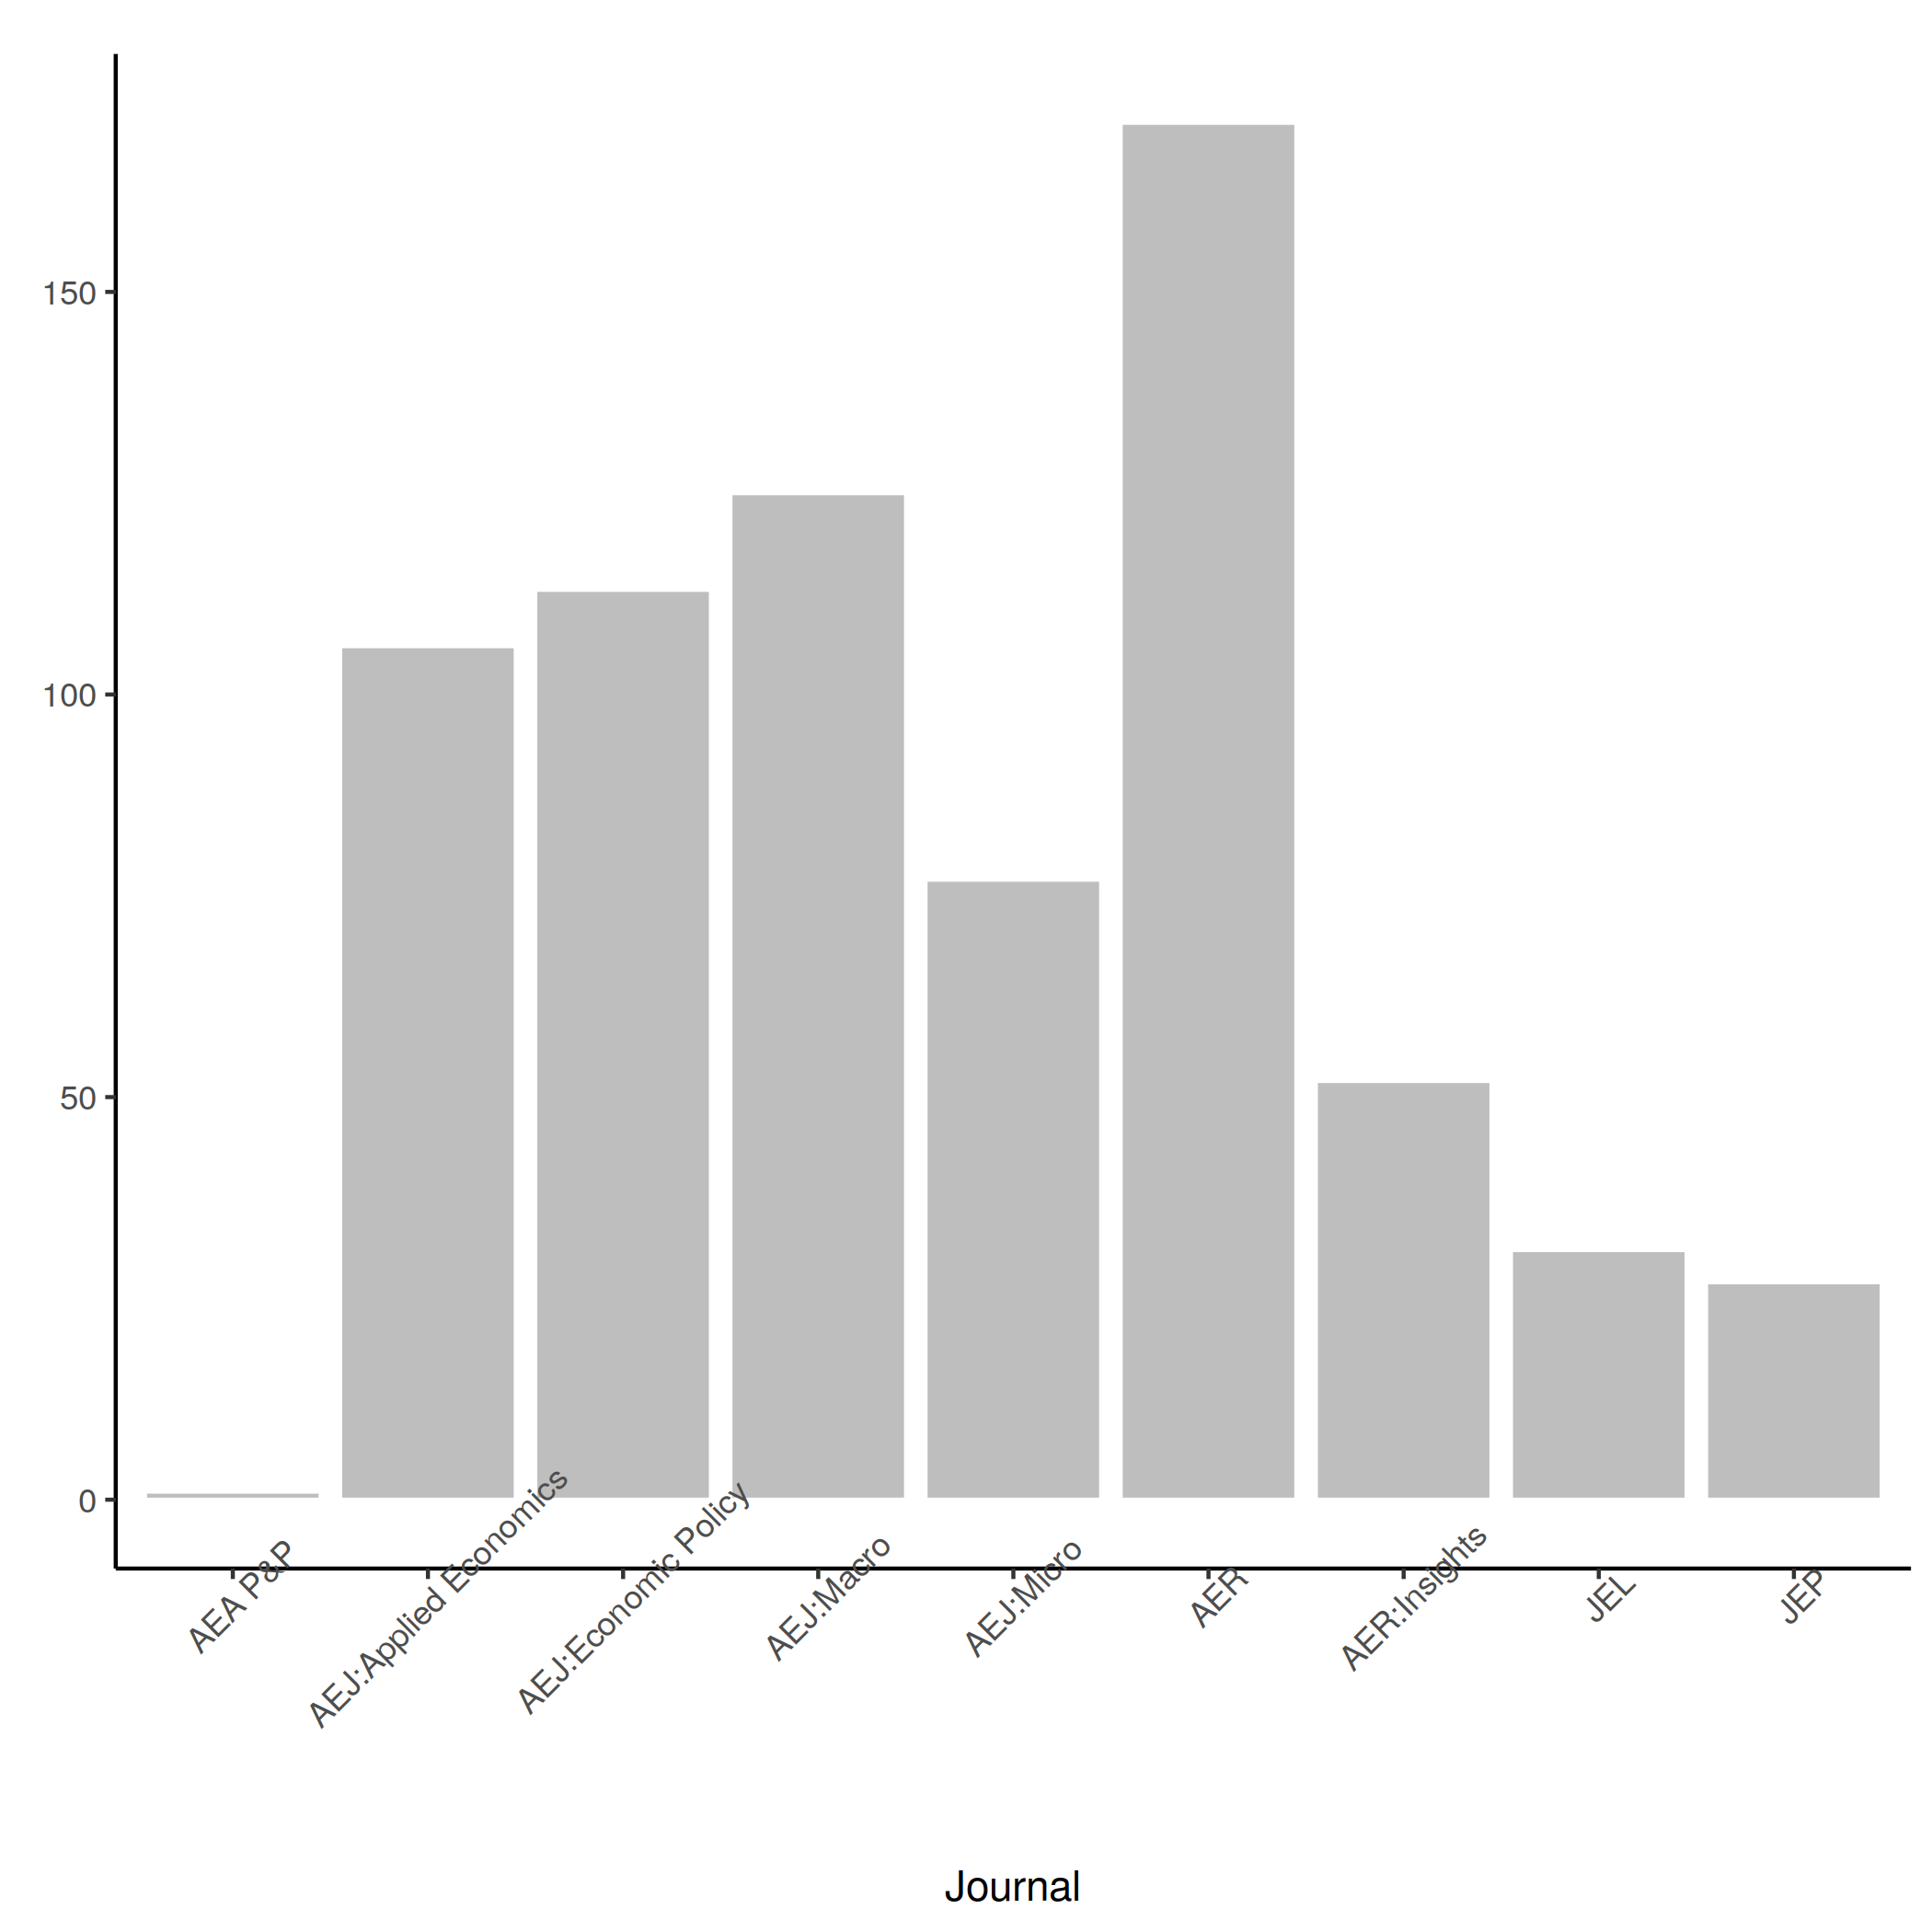
\includegraphics[height=0.4\textheight]{images/n_assessments_journal_plot.png}
    \caption{Number of assessments}
    \label{fig:pre:assessments_journal}
\end{figure}



\begin{figure}
    \centering
%    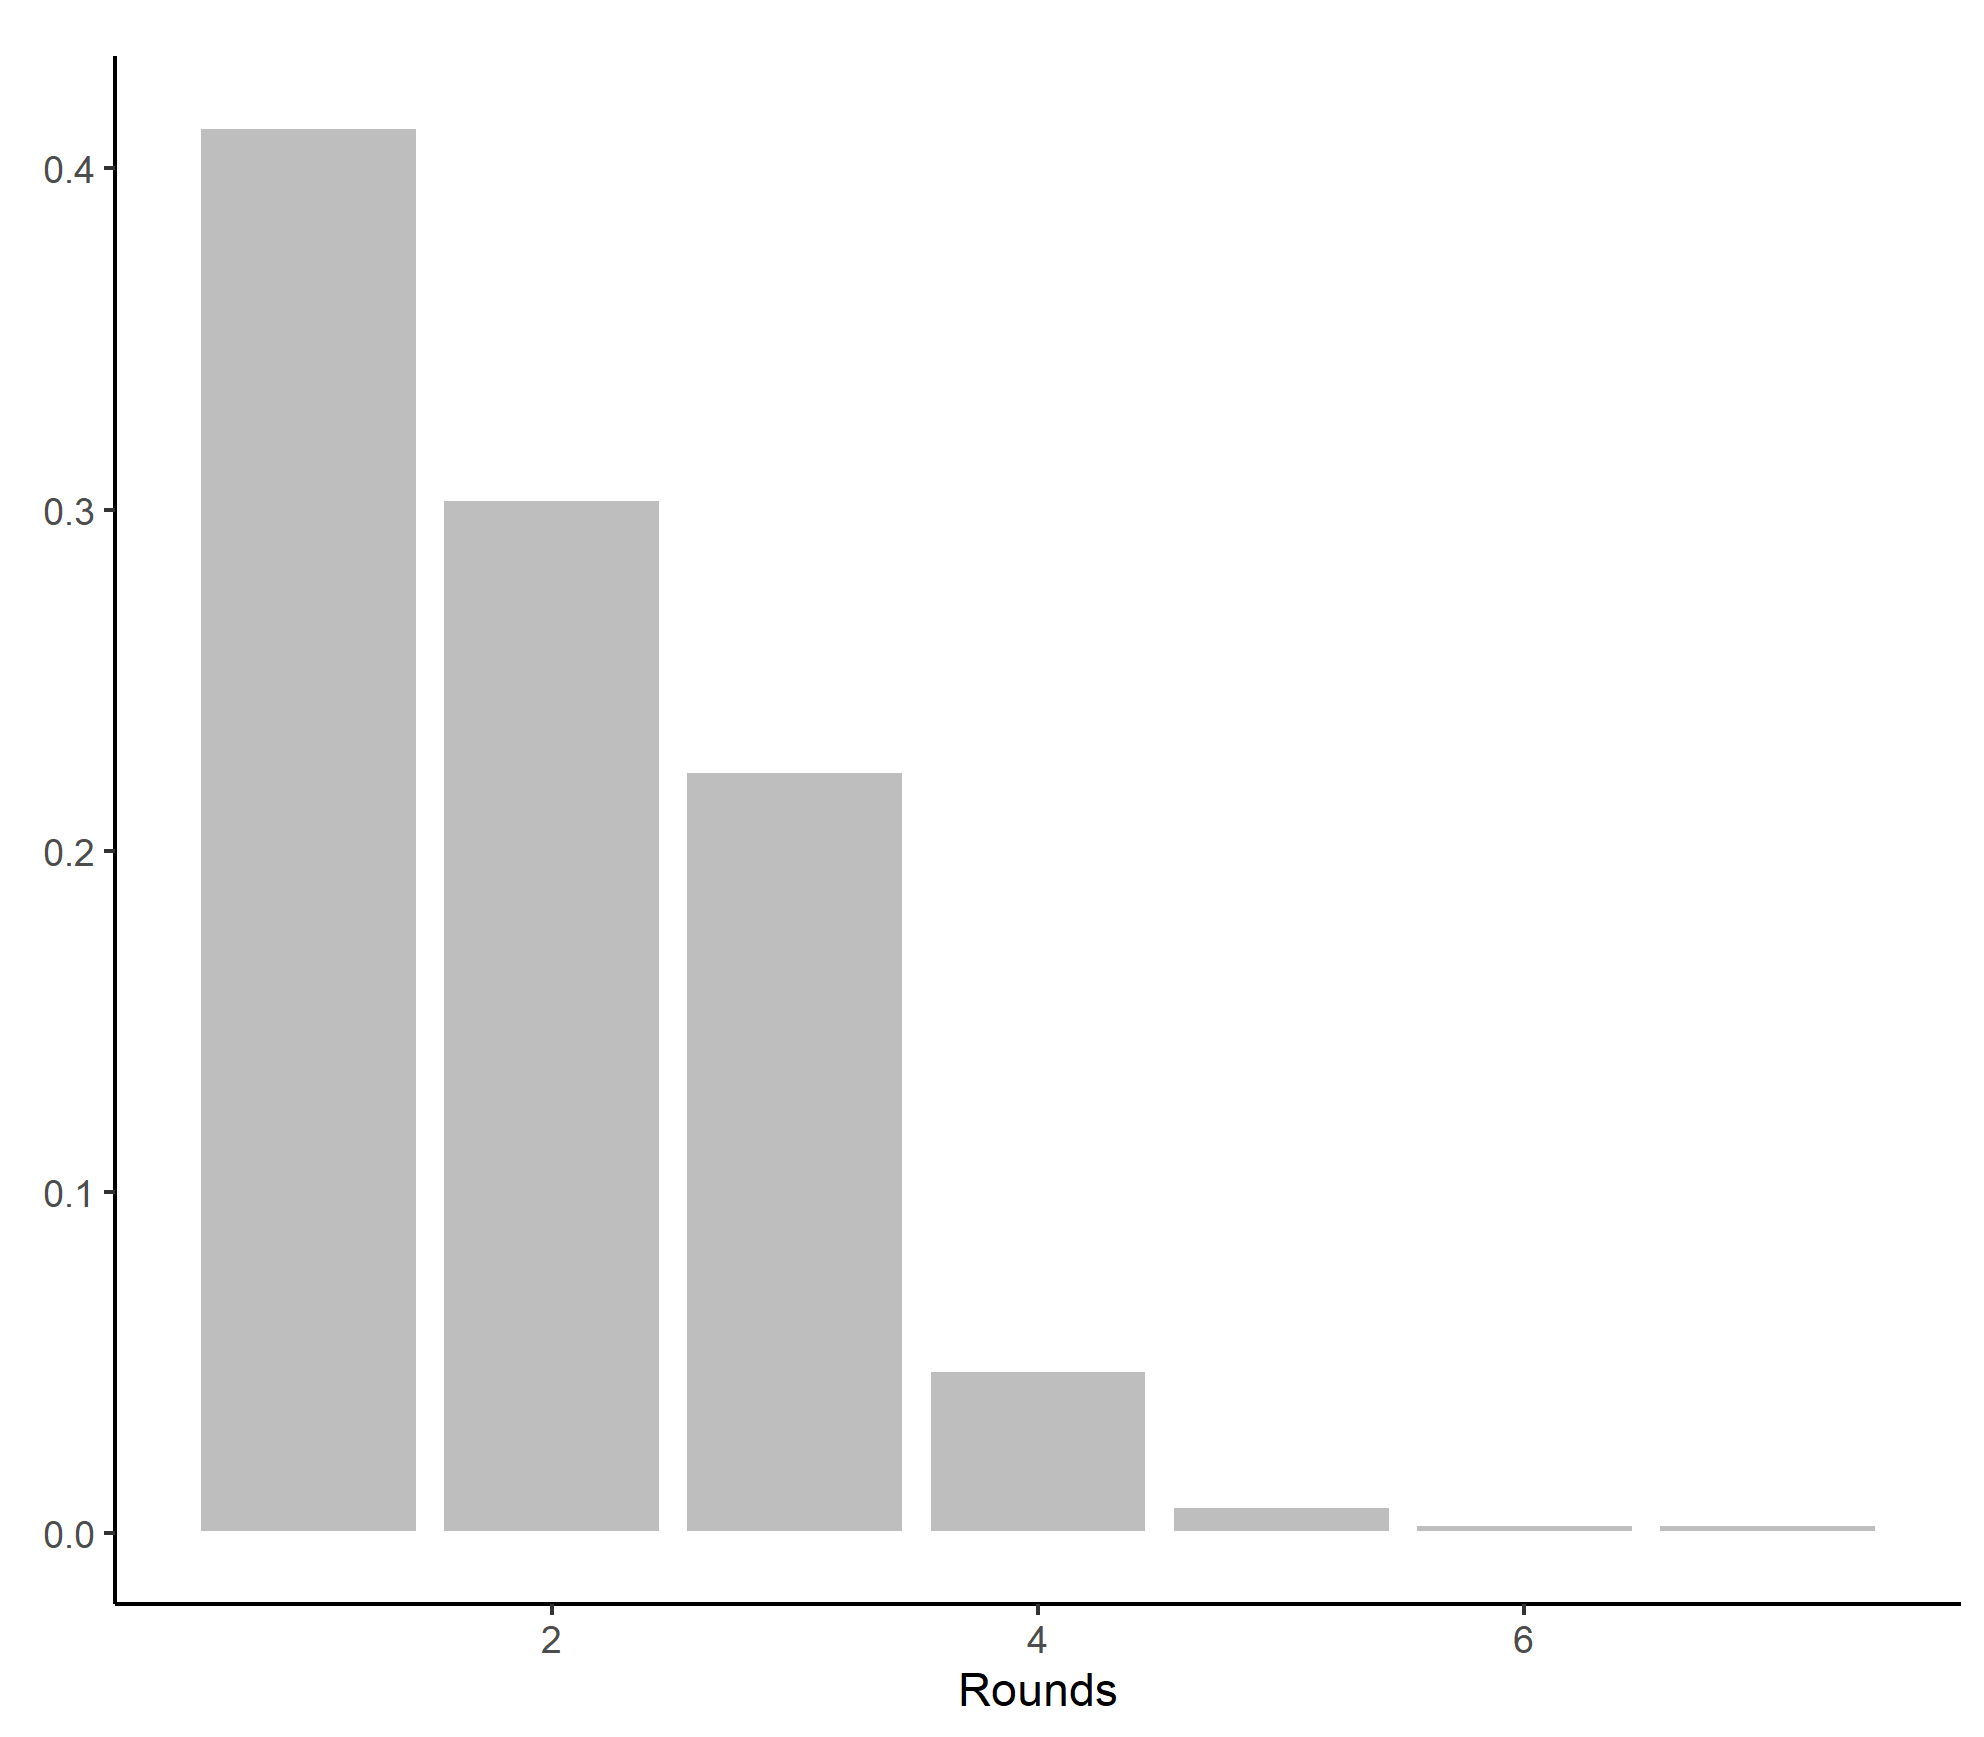
\includegraphics[height=0.4\textheight]{images/n_rounds_plot.png}
    \caption{Assessment rounds for completed manuscripts}
    \label{fig:pre:rounds}
\end{figure}

\begin{figure}
    \centering
%    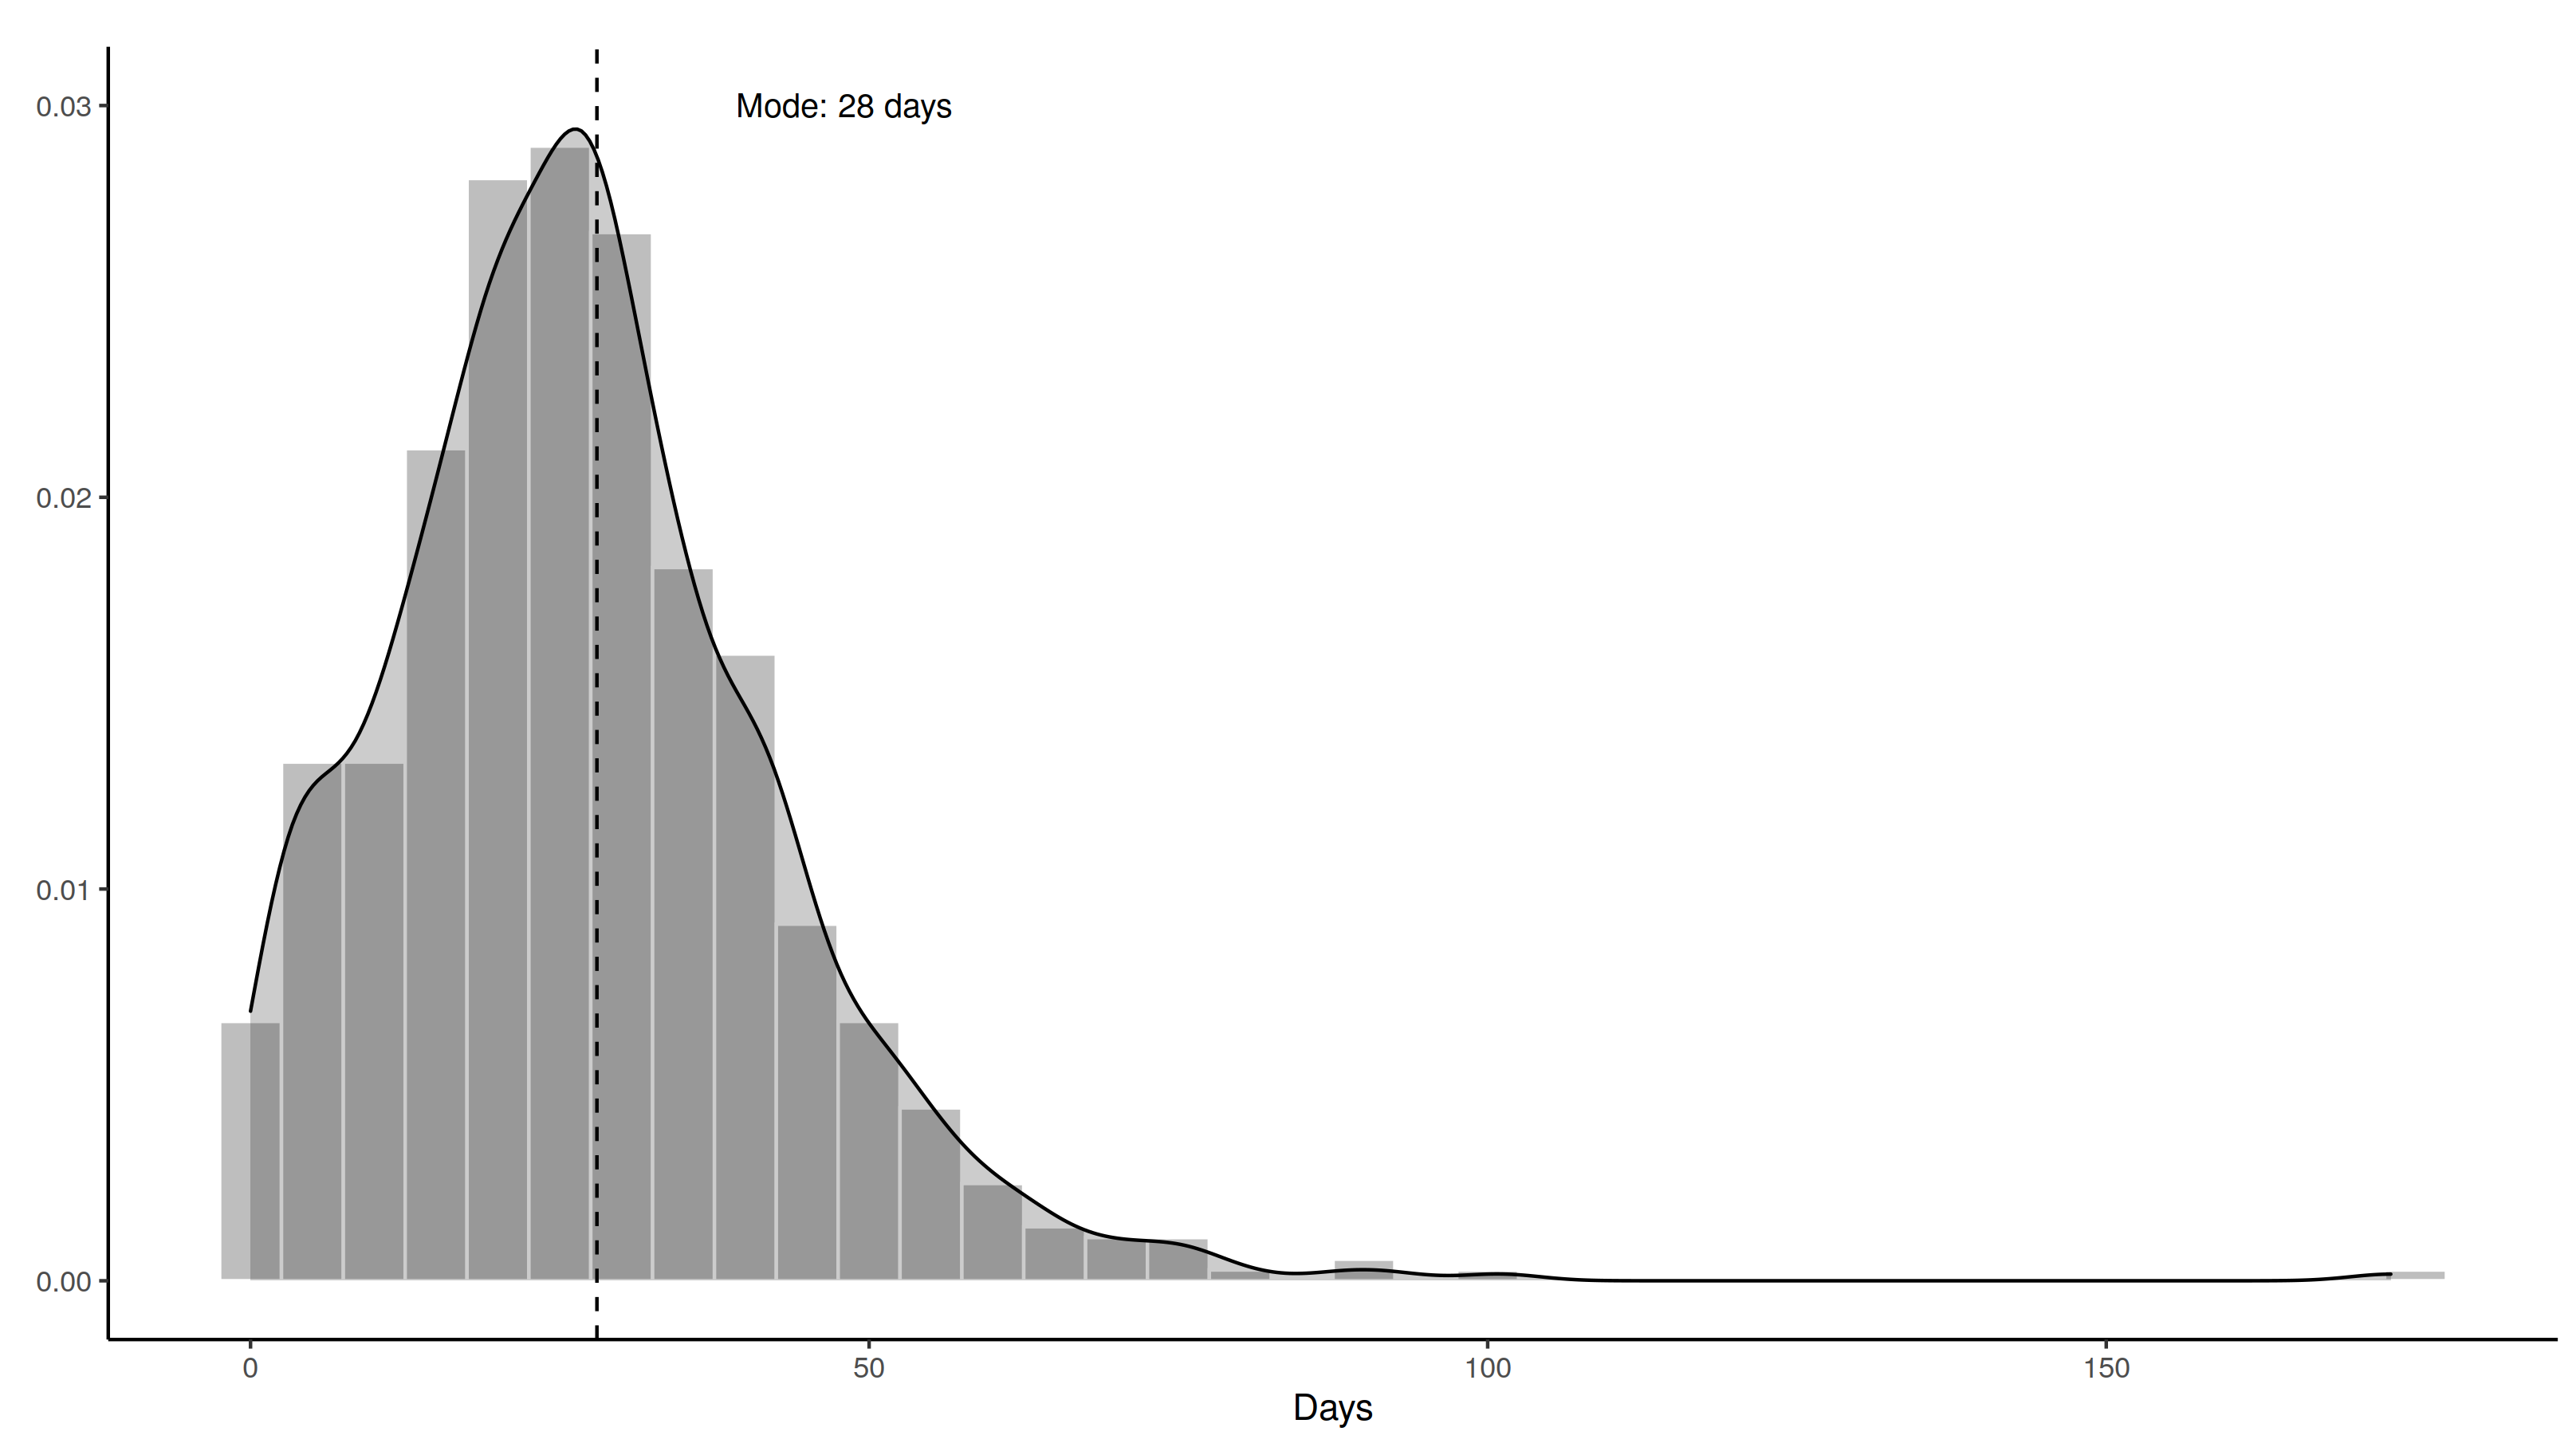
\includegraphics[height=0.4\textheight]{images/revision_round_length_hist.png}
    \caption{Length of an assessment round in days}
    \label{fig:pre:round_length}
\end{figure}

\begin{figure}
    \centering
%    \includegraphics[height=0.4\textheight]{images/total_length_hist.png}
    \caption{Length of revisions for completed manuscripts}
    \label{fig:pre:revision_length}
\end{figure}




\begin{figure}
    \centering
%    \includegraphics[height=0.4\textheight]{images/author_response_hist.png}
    \caption{Author response time}
    \label{fig:pre:author_response_time}
\end{figure}

\begin{quote}
    Issues with pre-publication verification
\end{quote}

\end{comment}

\paragraph{Self-corrections}

We often find that authors find other errors than those the replication team identified. For instance, the manuscript figures might have come from an earlier version of the dataset, or from an earlier run of the code sequence with slightly different parameters. In other cases, while reviewing issues found by our replication team, authors correct econometric errors, which our process is not designed to find. 

\paragraph{Computational issues}

Numerical differences (Matlab versions, seeds) see \url{https://it.mathworks.com/matlabcentral/answers/
422349-fmincon-in-new-matlab-version-gives-different-results} as well. Cite the old papers. In some cases, the underlying feature leading to numerical differences is a subtle fragility of the optimization algorithm, or multiple distinct yet close optima that do not fundamentally affect the results.

Fortran challenges (manual compilation instructions, non-open source compile, no Makefiles, no parameter files).

GIS challenges (not considered use of "data", often not described at all, or mostly manual tasks when using ArcGIS - very little python with ArcGIS). 

Robustness checks that are manual

\paragraph{Delays} A recurring concern expressed by editors and staff members was the potential for   delays in publication, due to the verification process. The data presented here indicates that concerns of about a delay in the time-to-publication remain valid, though we have no evidence at this time that the overall time to publication has increased --- the first articles that completed the entire pre-publication verification process were published in late January 2020, after the analysis in this article was completed.

We are addressing these concerns in a variety of ways. First, the current set of manuscripts moving through the assessment process did not anticipate the process --- the manuscripts were written and refereed prior to the July announcement. They thus could not incorporate stronger guidance as easily as future submissions will be able to. Second, we are expanding guidance, as well as preparing template README and project structures that will assist future manuscript submissions to be more rapidly compliant with the \ac{DCAP}, ideally in a first pass. This may include stronger requirements about the information to be provided by authors, including detailed information about the length of time it takes to execute the computer code.
Third, there is anecdotal evidence that other factors affecting the time-to-publication have been reduced, due to the move to conditional acceptance. Thus, manuscript materials are being completed earlier than before. 

We note that none of the \jiramcs{} manuscripts we assessed had  fundamental flaws --- all problems identified so far have been fixable (and fixed). 

\subsection{Migrating Historical Supplements}
\label{sec:migration}

We initially migrated the bulk of historical data (and code) supplements, from ZIP files stored on AEA servers to the \aeadcr{}. As noted earlier, for many of these deposits, we have successfully requested assistance from several hundred authors to update the metadata, improving presentation and findability. A few hundred replication packages are still pending migration, pending reconciliation of duplicates and large-file limitations. Upon demand from readers, we have also sometimes reached out to authors to request materials from articles which were published prior to the original publication of a data availability policy. 

% report on UMich metadata project

\subsection{Improving the \aeadcr{}}
\label{sec:improvingaeadcr}

We continually assess the performance of the \aeadcr{}. In collaboration with ICPSR, we have increased the default quota from 2GB to 30GB, streamlining the ability of researchers to deposit large replication packages.\footnote{It was previously possible to deposit large replication packages greater than 2GB, but required manual adjustments, resulting in delays and occasionally confusion.} A new workflow has been developed, which provides greater clarity to journal managers on the back-end, and prevents errors that users frequently made. It lays the groundwork for further enhancements in the future. 

% distribution of sizes - email from Jared

\begin{figure}
    \centering
    %\includegraphics{} 
    PLACEHOLDER - 
    \caption{Size distribution of replication packages deposited between  \firstday{} to \lastday{}}
    \label{fig:size_packages}
\end{figure}



\section{Task 3: Working with Other Providers of Scientific Infrastructure to Improve Support for Documenting Provenance and Replicability}
\label{sec:coordination}

An important component of the AEA Data Editor's position is to interact with other providers of scientific infrastructure. This involves other publishers and journals, archives such as ICPSR, providers of restricted or proprietary data, the AEA RCT Registry, metadata harvesters, and third-party verification services. 
% for exec summary: Also briefing to staff members of the House and Senate Science committees.

\subsection{Highlighting Data Resources}

NEW: See Ganapati \url{https://www.aeaweb.org/articles?id=10.1257/mic.20190029} and Harari \url{https://www.aeaweb.org/articles?id=10.1257/aer.20171673} data extracts, deposits. Also 200GB of NASA data, IPUMS terms of use, citations, and conundrum of copying data when (easy) retrieval from the original provider is not possible.

\subsection{Economics Journals}

We have coordinated with other data editors conducting similar activities at other journals. In 2019, both the \ac{ReStud} and the \ac{EJ}  appointed data editors, tasked among other things with pre-publication verification. The \ac{CJE} is currently revising its \ac{DCAP}. The \ac{JASA} is expanding the scope of its pre-publication verification to all sections of the journal. In all cases, either the AEA Data Editor or an ad-hoc group of ``Social Science Data Editors'' initiate by the AEA Data Editor, was consulted. The ``Social Science Data Editors'' group includes  editors from journals that do not (yet) have a pre-publication verification service. A  \urlcite{socialsciencedataeditors.github.io}{website} provides examples, checklists, and links to training materials, to assist authors in  improving data and code archives prior to submission, regardless of the journal they may be submitting to.

\subsection{Search services, text mining access}
As noted earlier, the move of supplements into the openICPSR-supported repository enables broad dissemination of metadata on supplements. Among others, Google Dataset Search harvests and then displays such metadata. Staff from openICPSR and the AEA Data Editor have been discussing informally with the Google Dataset Search team on how to correctly display metadata as it moves through the various scrapers. 

Over the course of the past year, the AEA has been approached by two research projects that wished to use the full-text versions of AEA articles to enhance the linkage between articles and data. We worked with these teams to establish a policy by which they could legally access the full archive of articles, but also subsequently make their work available to others. AEA counsel is currently working on a full-fledged data and text mining policy.

\subsection{Third-party verification services}
\label{sec:3rdparty}

\begin{quote}
    Write a lot here.
\end{quote}
We have started discussions with third-party verification services. In particular, we have trialled using their services, instead of our in-house team, to conduct assessments. This aligns with the discussions among editors about resources and scalability of assessments, and with the educational outreach, which some of these services also conduct. Part of the effort consists in aligning the criteria used by these services with those of the various journals.

\subsection{Commercial providers}

Highlight exemplary redistribution agreement at ESRI. Highlight in all cases the need to have access rights for pre-production verification, including to the same access mechanisms. 

\subsection{Non-commercial providers of restricted-access data}

Increased provision of data citations, clear license/ usage rights. Ongoing work. Briefings of US, Canadian, German, French, UK restricted access centers. Some providers have also reached out to inquire pro-actively how to improve their access mechanisms, distribution mechanisms, and documentation thereof.

\section{Task 4: Working with the Economics Community to Enhance and Broaden Education on Replicable Science}

\begin{quote}
    write about participation of other journals, as well as nascent efforts around Data-PASS and RDA.
\end{quote}

From the preliminary verification work has emerged a clear indication that education and training is critical for the adoption of reproducible methods. We are expanding the support materials, and are adapting them to each discipline's idiosyncratic methods. Training materials will be made available by various organizations, with input from the AEA Data Editor. The \urlcite{https://aeadataeditor.github.io/aea-de-guidance/}{AEA Data Editor's website} as well as the website of the \urlcite{https://social-science-data-editors.github.io/guidance/}{Social Science Data Editors} are being regularly updated with additional guidance, and will hopefully allow authors to be responsive to various journals' \ac{DCAP}.

\section{Data and Code Availability Statement}
\label{sec:dcas}

All data and code used to generate figures and tables in this article can be found at \citet{E117884V1}, with some data archived as \citet{E117873V1} and \citet{E117876V1}. Data on the AEA RCT Registry was extracted by JT and KW from internal systems, but can now be downloaded directly \citep{DVN/DFMLIU_2020}. The data provided here as part of \citet{E117884V1} may differ.

\FloatBarrier
% Remove or comment out the next two lines if you are not using bibtex.
%
% NOTE: Do not modify the AEADataEditor.bib manually!
%
\bibliographystyle{aea-mod}
\bibliography{paper,references}

% The appendix command is issued once, prior to all appendices, if any.
\appendix

%\input{appendix.tex}


\end{document}

